\chapter{Description microscopique des bois résineux}\label{resineux}

\begin{abstract}
Ce chapitre décrit chacun des types de cellules rencontrés chez les arbres résineux. Nous nous attardons aussi à certaines caractéristiques anatomiques, comme les ponctuations des champs de croisement, qui permettent d'identifier les espèces.
\end{abstract}

\minitoc

\section{Introduction}

La caractéristique essentielle du bois des résineux (gymnospermes) est l'absence de cellules spécialisées pour la conduction de la sève brute tel qu'on en retrouve chez les feuillus. La sève brute circule par les trachéides longitudinales qui jouent à la fois un rôle de support mécanique et de conduction.\\

Le bois des résineux possède une structure simple composée essentiellement de trois types de cellules :

\begin{enumerate}
\item Les trachéides longitudinales;
\item Les trachéides transversales;
\item Les parenchymes :
	\begin{itemize}
	\item Parenchyme de rayon;
	\item Cellules épithéliales;
	\item Parenchyme longitudinal
	\end{itemize}
\end{enumerate}

\section{Cellules orientées longitudinalement}

\subsection{Trachéides longitudinales}

Les trachéides longitudinales sont les plus longues cellules que l'on retrouve chez les bois résineux et feuillus. Elles représentent environ 92\% du volume du bois. Elles ont deux fonctions principales, soit le support mécanique de la tige et la conduction de la sève brute. Leur longueur varie de 3 à 7 mm environ en fonction des espèces (voir Tableau~\ref{tab:diam_long}).\\

En plan transversal, les trachéides longitudinales sont disposées en files radiales. Ceci est spécifique aux résineux, les feuillus présentant une disposition plutôt aléatoire. Cette disposition en files radiales s'explique par le fait que le diamètre tangentiel des trachéides longitudinales change peu ou pas, du bois initial au bois final. Par contre, le diamètre radial des trachéides diminue du bois initial au bois final et l'épaisseur des parois cellulaires augmente. La section des trachéides longitudinales est de forme plutôt hexagonale dans le bois initial et de forme rectangulaire dans le bois final.

\begin{table}[ht]
\centering
	
	\begin{tabular}{l c c}
	\hline
	\bf Espèce	& \bf $\varnothing$ tangentiel (\micro m)& \bf Longueur (mm) \\
	\hline\hline
	Séquoia (\textit{Sequoia sempervirens}) & 50-80 & 7.0 \\
	Pin à encens (\textit{Pinus taeda})  &  35-60 &  4.3\\
	Sapin Douglas (\textit{Pseudotsuga menziesii})  & 35-55 & 3.4 \\
	Sapin baumier (\textit{Abies balsamea})  & 30-50 & 3.3 \\
	Pin blanc \textit{(Pinus strobus})  & 25-45 &  3.5 \\
	Mélèze laricin (\textit{Larix laricina})  & 30-45 & 3.0 \\
	Épinette noire (\textit{Picea mariana})  & 25-30 & 3.5 \\
	Épinette blanche (\textit{Picea glauca})  & 25-35 & 3.3 \\
	Genévrier rouge (\textit{Juniperus virginiana})  & 20-35 & 2.2 \\
	If de l'Ouest (\textit{Taxus brevifolia}) & 15-25 &  2.3\\
	\hline
	\end{tabular}

\caption{\label{tab:diam_long} Dimensions des trachéides de quelques bois résineux (d'après \cite{panshin1980textbook}}
\end{table}

La transition du bois initial au bois final varie en fonction des espèces. Par exemple, elle est graduelle chez l'épinette (\textit{Picea spp.}) et abrupte chez le sapin Douglas (\textit{Pseudotsuga menziesii}) (Figure~\ref{transition}).

\begin{figure}[h]
\centering
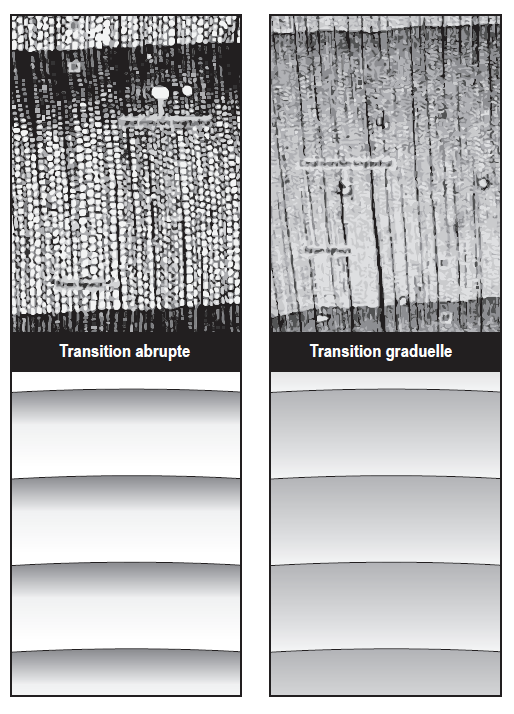
\includegraphics[scale=0.6]{img/ch3_transition}
\caption{Illustration de la différence entre une transition abrupte chez le Douglas (\textit{Pseudotsuga menziesii}) et graduelle chez l'épinette (\textit{Picea spp.}) (grossissement : $\times$40) du bois initial au bois final. Image préparée par Julie Ferland pour \cite{achim2010dendroecologie}}
\label{transition}
\end{figure}

\subsubsection{Dimensions des trachéides longitudinales}

Le diamètre tangentiel des trachéides est un caractère héréditaire, donc peu variable à l'intérieur d'une espèce. Ce caractère défini les bois résineux à texture fine ou grossière (Figure~\ref{fig:texture}). Par exemple, le bois de séquoia présente une texture grossière avec des trachéides longitudinales d'un diamètre tangentiel moyen d'environ 80 \micro m. À l'opposé, le bois du if de l'Ouest (\textit{Taxus brevifolia}) a une texture fine avec des trachéides longitudinales d'un diamètre tangentiel moyen d'environ 25 \micro m. Plusieurs bois résineux commerciaux ont une texture moyenne avec des trachéides longitudinales d'un diamètre tangentiel variant de 30 à 45 \micro m (Tableau~\ref{tab:diam_long}). On remarque que la longueur des trachéides longitudinales est généralement corrélée avec le diamètre tangentiel, c'est-à-dire que les bois à texture grossière possèdent également les plus longues trachéides longitudinales.

\subsubsection{Épaississements spiralés}

Les épaississements spiralés sont des épaississements de la paroi tertiaire (S\sub{3}) des trachéides, disposés du côté du lumen (Figure~\ref{fig:epaississ}). Ils sont toujours présents chez les trachéides longitudinales et transversales du bois de sapin Douglas et sont utilisés comme critère d'identification pour cette espèce.\\

L'angle que font les épaississements avec l'axe longitudinal de la trachéide est approximativement le même que celui des microfibrilles de la paroi S\sub{3}. On distingue les épaississements en \og S \fg  et les épaississements en \og Z \fg  en fonction de l'orientation de la spirale lorsqu'on l'observe en plan longitudinal-radial ou longitudinal-tangentiel. 

%image à refaire avec une meilleure résolution
\begin{figure}[h]
\centering
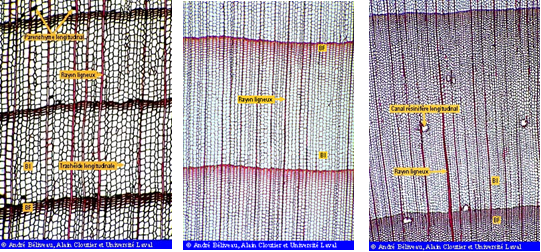
\includegraphics[scale=0.7]{img/texture}
\caption{De gauche à droite : Bois à texture grossière (séquoia); bois à texture moyenne (sapin baumier); bois à texture fine (épinette) (grossissement $\times$40).}
\label{fig:texture}
\end{figure}

\begin{figure}[h]
\centering
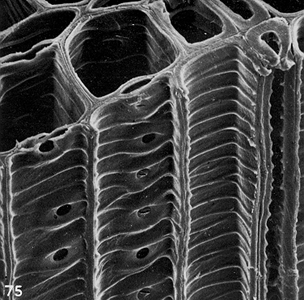
\includegraphics[scale=1]{img/epaississements}
\caption{Épaississements spiralés en S chez le sapin Douglas (\textit{Pseudotsuga menziesii}) (tiré de \cite{butterfield2012three}; grossissement $\times$850)}
\label{fig:epaississ}
\end{figure}

\subsection{Files de trachéides}

Les files de trachéides sont constituées de courtes trachéides longitudinales dotées de parois terminales. Elles possèdent des ponctuations aréolées, ce qui permet de les différencier des parenchymes longitudinaux. Ces trachéides courtes peuvent être considérées comme des cellules transitoires entre les trachéides longitudinales d'une part et les parenchymes longitudinaux et les cellules épithéliales d'autre part. Lorsqu'elles sont présentes, les files de trachéides sont souvent situées au voisinage des canaux résinifères, à la marge des cernes annuels ou au voisinage des canaux résinifères traumatiques. En Amérique du Nord, on les retrouve parfois chez les mélèzes (\textit{Larix spp.}) (Figure~\ref{fig:file}), le sapin Douglas et le séquoia (\textit{Sequoia sempervirens}).

\subsection{Parenchymes orientés longitudinalement}

Les parenchymes sont des cellules ayant pour fonction la sécrétion des résines ou la réserve de substances nutritives. Leur paroi cellulaire a une structure différente de celle des trachéides puisqu'on a soit une paroi primaire mince, soit une paroi primaire épaissie qui a l'allure d'une paroi secondaire. On rencontre deux types de parenchymes orientés longitudinalement chez les résineux : 1) le parenchyme longitudinal et 2) le parenchyme épithélial (ou cellules épithéliales).

\begin{figure}[h]
\centering
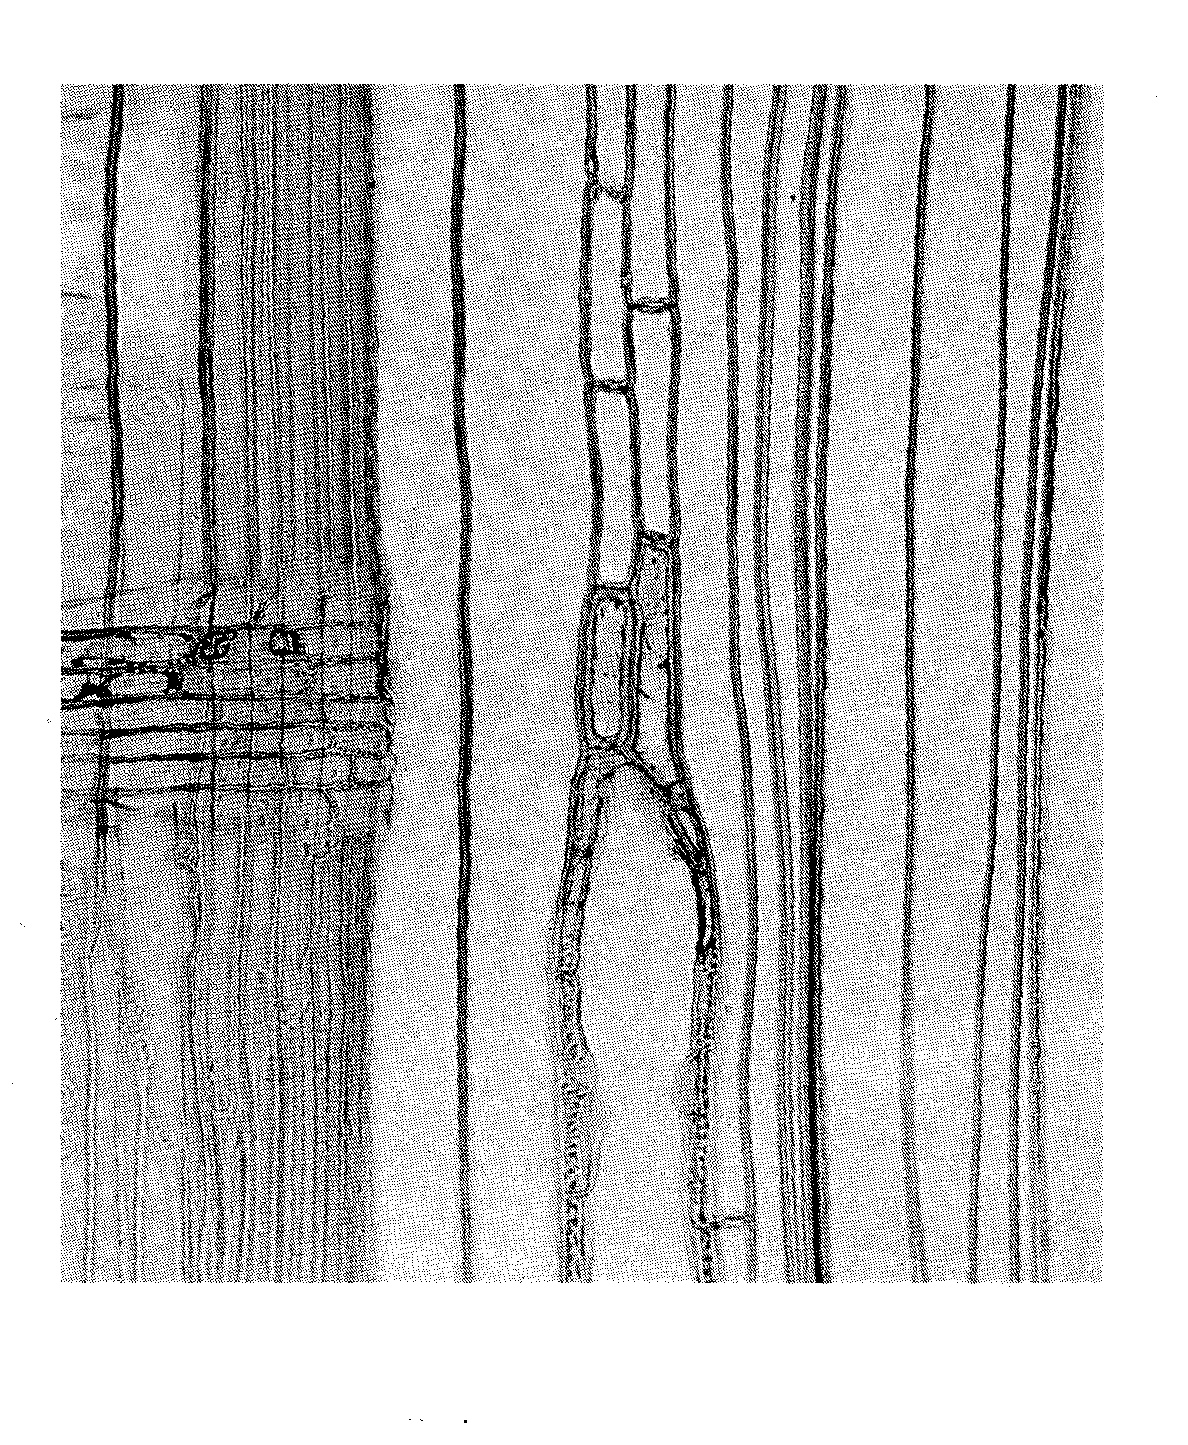
\includegraphics[scale=0.2]{img/file}
\caption{File de trachéides chez le mélèze de l'Ouest (\textit{Larix occidentalis}) (adapté de \cite{panshin1980textbook}}
\label{fig:file}
\end{figure}

\subsubsection{Parenchyme longitudinal}

Contrairement aux feuillus, le parenchyme longitudinal n'est pas très fréquent ni abondant chez les résineux. On le rencontre toutefois chez certaines espèces où il prend la forme de files orientées longitudinalement. Il sert alors de tissu de réserve. Comme c'est toujours le cas entre les parenchymes, les ponctuations sont simples au niveau des parois terminales, c'est-à-dire à l'interface entre deux cellules de parenchyme. Les parois terminales sont dites lisses ou noduleuses selon que les ponctuations simples forment des nodules ou non.\\

Le parenchyme longitudinal n'est jamais présent chez le genre \textit{Pinus}. Il est sporadiquement présent chez les genres \textit{Larix}, \textit{Pseudotsuga}, \textit{Tsuga} et \textit{Abies}. Il est relativement abondant chez les genres de la famille des Cupressaceae (\textit{Thuja, Chamaecyparis, Cupressus, Calocedrus,} et \textit{Juniperus}). Toutefois, il est abondant chez les genres de la famille des Taxodiaceae (\textit{Sequoia} et \textit{Taxodium}). Le parenchyme longitudinal chez le séquoia est présenté à la figure~\ref{fig:par_long}.\\

\subsection{Parenchyme épithélial et canaux résinifères longitudinaux}

Les cellules de parenchyme épithélial sécrètent la résine chez les résineux. Elles recouvrent les canaux résinifères longitudinaux et transversaux des bois résineux qui en possèdent. Un canal résinifère est en réalité un espace intercellulaire, c'est-à-dire une cavité recouverte de cellules épithéliales. Les cellules épithéliales forment l'épithélium qui peut avoir plusieurs cellules d'épaisseur. L'épaisseur des cellules épithéliales varie d'une espèce à l'autre. On les qualifie de cellules épithéliales à paroi mince (Figure~\ref{fig:epth_mince}) ou de cellules épithéliales à paroi épaisse (Figure~\ref{fig:epth_epaisse}). Le tableau~\ref{tab:mince_epaisse} présente les principales caractéristiques de quelques bois résineux d'Amérique du Nord en ce qui concerne les canaux résinifères.


\begin{figure}[h]
\centering
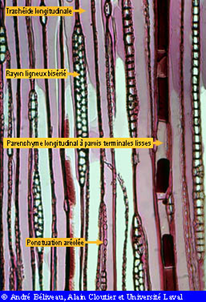
\includegraphics[scale=0.7]{img/parenchyme_long}
\caption{Parenchyme longitudinal à parois terminales lisses en coupe longitudinale-tangentielle chez le séquoia (\textit{Sequoia sempervirens}) (grossissement $\times$100).}
\label{fig:par_long}
\end{figure}

\begin{figure}[h]
\centering
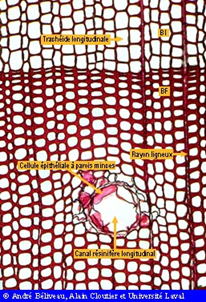
\includegraphics[scale=0.7]{img/epith_mince}
\caption{Canal résinifère longitudinal et cellules épithéliales à paroi mince chez le pin blanc (\textit{Pinus strobus}) (grossissement $\times$100)}
\label{fig:epth_mince}
\end{figure}


\begin{figure}[h]
\centering
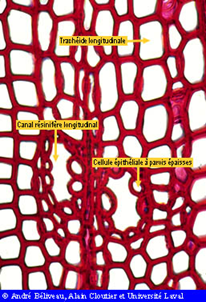
\includegraphics[scale=0.7]{img/epith_epaisse}
\caption{Canal résinifère longitudinal et cellules épithéliales à paroi épaisse chez l'épinette \textit{(Picea spp.)} (grossissement : $\times$400)}
\label{fig:epth_epaisse}
\end{figure}

\begin{table}[ht]
	\centering
	
	\begin{tabular}{l c c}
		\hline
		\bf Sans canaux résinifères normaux	& \multicolumn{2}{c}{\textbf{Avec canaux résinifères normaux}}\\
		& \bf cell. épith. à parois minces & \bf cell. épith. à parois épaisses\\
		\hline\hline
		Pruches \textit{(Tsuga spp.)} &	Pins \textit{(Pinus spp.)} &	Épinettes \textit{(Picea spp.)}\\
		Sapins \textit{(Abies spp.)} & & Mélèzes \textit{(Larix spp.)}\\
		Genévrier rouge \textit{(J. virginiana)} & & Sapin Douglas \textit{(P. menziesii)}\\
		Séquoia \textit{(Sequoia sempervirens)} &&\\
		Thuyas \textit{(Thuja spp.)}&&\\
		\hline
	\end{tabular}
	
	\caption{\label{tab:mince_epaisse} Présence ou absence des canaux résinifères normaux chez quelques bois résineux d’Amérique du Nord}
\end{table}

Les cellules épithéliales à paroi mince et à paroi épaisse présentent certaines particularités. Les cellules épithéliales à paroi mince des pins n'ont pas de ponctuations et ne sont pas lignifiées. Les cellules épithéliales à paroi épaisse des épinettes, des mélèzes et du sapin Douglas ont des ponctuations et sont lignifiées.

\subsection{Canaux résinifères normaux ou traumatiques}

Les canaux résinifères sont qualifiés de normaux ou de traumatiques. Les canaux résinifères normaux sont toujours présents chez les espèces où ils sont caractéristiques. Ces canaux résinifères sont présents en direction longitudinale et en direction radiale dans les rayons fusiformes.\\

Les canaux résinifères traumatiques apparaissent chez des arbres ayant subi une blessure mécanique du cambium, une attaque d'insectes ou toute autre source de stress. Ils peuvent être transversaux ou longitudinaux mais rarement les deux pour un échantillon donné. Ils peuvent être présents chez des espèces qui n'ont pas de canaux résinifères normaux comme les pruches et les sapins. Les cellules épithéliales des canaux résinifères traumatiques sont toujours à paroi épaisse et sont lignifiées.

\section{Cellules orientées transversalement}

On rencontre trois types de cellules orientées transversalement dans le xylème des résineux qui sont toutes présentes des les rayons ligneux: 1) les parenchymes de rayon; 2) les trachéides transversales et 3) les cellules épithéliales.

\subsection{Parenchymes de rayon et rayons ligneux}

Les cellules des parenchymes de rayon ont des parois cellulaires minces. Il s'agit de paroi primaire plus ou moins épaissie. Les ponctuations entre ces cellules sont de type simple. Les ponctuations du plan longitudinal-radial des parenchymes de rayon en contact avec les trachéides longitudinales sont appelées champs de croisement (Figure~\ref{fig:croisement}). La forme des ponctuations semi-aréolées que l'on retrouve dans les champs de croisement est importante pour l'identification des bois résineux.\\

Les parenchymes de rayon forment les rayons qui sont disposés en direction radiale. Les cellules de parenchyme de rayon du bois d'aubier sont vivantes et celles du bois de duramen sont mortes. Les rayons ligneux traversent le xylème et le phloème et sont utilisés pour le transport de la sève élaborée du phloème vers les parenchymes vivants de l'aubier. Les rayons ligneux ne contenant qu'une cellule de large en plan longitudinal-tangentiel sont dits unisériés. Si on a deux cellules de large, on a alors des rayons ligneux bisériés. Dans la plupart des cas, les rayons sont unisériés chez les résineux. La hauteur des rayons varie entre les espèces. Elle est de 40 à 60 cellules de hauteur (0,5 à 1 mm) chez le séquoia, de 10 à 15 cellules en moyenne et peut descendre à moins de 6 cellules (0,3 mm) chez le genévrier. Le volume moyen des rayons est d'environ 7\% du volume total du bois chez les résineux.

\begin{figure}[h]
	\centering
	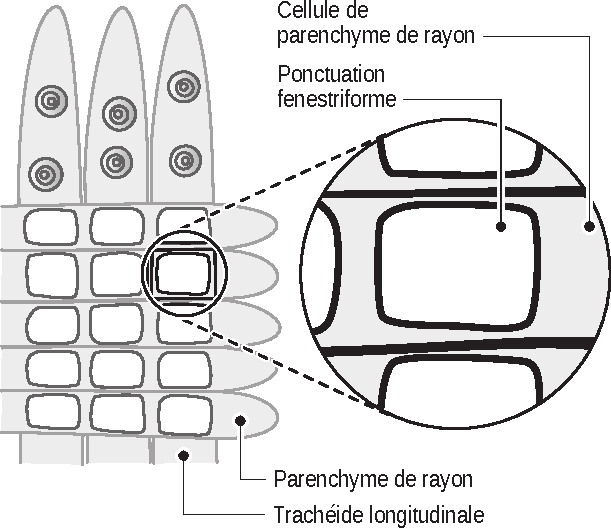
\includegraphics[scale=0.8]{img/ch3_croisement}
	\caption{Le champs de croisement sont constitués par l'interface entre des cellules de rayon et des trachéides dans le plan longitudinal-radial. Image préparée par Julie Ferland pour \cite{achim2010dendroecologie}}
	\label{fig:croisement}
\end{figure}

\subsection{Trachéides transversales et rayons fusiformes}

Les trachéides transversales sont présentes chez plusieurs résineux. Ce sont des cellules mortes orientées radialement et associées aux rayons ligneux. Elles possèdent des ponctuations aréolées tout comme les trachéides longitudinales, mais de plus petit diamètre. C'est d'ailleurs grâce à leurs paires de ponctuations aréolées qu'on peut facilement les distinguer des parenchymes de rayon (Figure~\ref{fig:trach_trans}).\\

Les trachéides transversales sont présentes chez les pins, les épinettes, les mélèzes, les pruches et le sapin de Douglas. On les retrouve sporadiquement chez les sapins et très rarement chez le séquoia, les thuyas et les genévriers.\\

Les trachéides transversales sont lisses ou dentées. Les trachéides transversales dentées (Figure~\ref{fig:dentees}) sont caractéristiques des groupes des pins durs (\textit{Pinus banksiana, Pinus resinosa, Pinus ponderosa}) et des pins du Sud (\textit{Pinus palustris, Pinus echinata, Pinus taeda, Pinus elliottii, Pinus rigida, Pinus serotina}, etc.).\\

Les parenchymes de rayon et le cas échéant les trachéides transversales vont parfois être associés à des canaux résinifères transversaux. Dans ce cas, on désigne cette structure comme étant un rayon fusiforme. On peut observer les rayons fusiformes en plan longitudinal-tangentiel (Figure~\ref{fig:fusiforme}). Ils permettent de s'assurer qu'il s'agit bien d'un bois possédant des canaux résinifères, car les canaux résinifères transversaux sont invariablement présents dans ce cas. Les rayons fusiformes contiennent donc les trachéides transversales, le parenchyme de rayon et les cellules épithéliales du ou des deux canaux résinifères présents.

\begin{figure}[h]
	\centering
	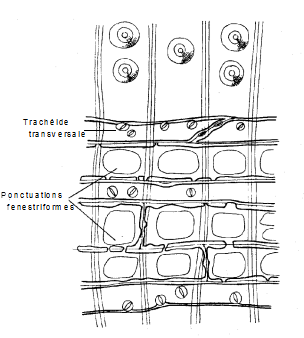
\includegraphics[scale=0.8]{img/ch3_Fahn_trach}
	\caption{Portion du plan longitudinal-radial d’un bois résineux montrant les parenchymes de rayon, les champs de croisement et les trachéides transversales (adapté de \cite{fahn1990plant})}
	\label{fig:trach_trans}
\end{figure}

\begin{figure}[h]
\centering
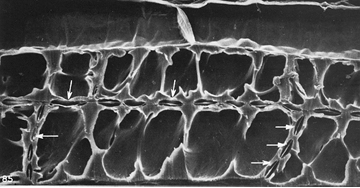
\includegraphics[scale=0.7]{img/ch3_dentees}
\caption{Trachéides transversales dentées en plan longitudinal-radial chez Pinus radiata (tiré de Butterfield et Meylan 1980) (grossissement : $\times$1500)}
\label{fig:dentees}
\end{figure}

\begin{figure}[h]
\centering
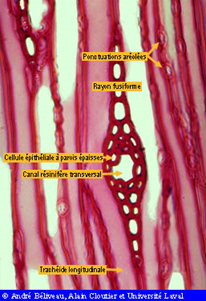
\includegraphics[scale=0.8]{img/ch3_fusiforme}
\caption{Rayon fusiforme en plan longitudinal-tangentiel chez l'épinette (Picea spp.) (Grossissement : $\times$400)}
\label{fig:fusiforme}
\end{figure}

Le nombre de rayons fusiformes est toujours inférieur au nombre de rayons unisériés. Par exemple, le ratio est de 1:25 chez le sapin Douglas, 1:40 chez les épinettes et 1:60 chez les mélèzes.\\

Les rayons unisériés sont dits homo-cellulaires s'ils ne sont constitués que de parenchymes de rayon ou que de trachéides transversales. Ils sont dits hétérocellulaires s'ils sont constitués d'un mélange des deux types de cellules.

\section{Ponctuations} %ajoute rimage comme au chapitre 4

Les ponctuations peuvent être définies comme une discontinuité dans la paroi cellulaire donnant naissance à une ouverture. Elles se présentent généralement deux à deux pour former une paire de ponctuations entre deux cellules servant au passage des liquides dans l'arbre vivant.
%
\subsection{Ponctuations parenchyme - parenchyme}

Les ponctuations que l'on retrouve entre les parenchymes et en particulier, entre les parenchymes de rayon, sont des paires de ponctuations simples (Figure~\ref{fig:ponctuations2}A).

\subsection{Ponctuations trachéide - trachéide}

Les ponctuations que l'on retrouve entre les trachéides sont des paires de ponctuations aréolées (Figure~\ref{fig:ponctuations2}B). Les paires de ponctuations inter-trachéales sont les plus nombreuses et les plus grosses sur les parois radiales des trachéides du bois initial. On peut avoir plus d'une ponctuation de large sur la face radiale des trachéides longitudinales : 

\begin{itemize}
\item texture fine (épinettes):	ponctuations unisériées;
\item texture moyenne (pins):	ponctuations bisériées;
\item texture grossière (séquoia):	3 à 4 ponctuations de large.
\end{itemize}

Les crassules sont des lignes foncées apparaissant sur les faces radiales des cellules autour des paires de ponctuations bisériées. Les ponctuations sur les parois tangentielles sont plus petites que sur les parois radiales et ne sont présentes que pour les dernières rangées de cellules du bois final. 

\subsection{Ponctuations trachéide - parenchyme}

Les ponctuations que l'on retrouve entre les trachéides et les parenchymes sont des paires de ponctuations semi-aréolées (Figure~\ref{fig:ponctuations2}C). Les ponctuations des champs de croisement sont de ce type et ont une importance particulière pour l'identification des bois de résineux. On distingue 5 types de ponctuations des champs de croisement qui sont illustrés à la figure~\ref{fig:ponctuations} et décrits ci-dessous. La figure~\ref{fig:pontuations_cote} montre des coupes de chacune de ces ponctuations qui pourront vous aider à comprendre ce que vous observerez au microscope.

\begin{figure}[h]
\centering
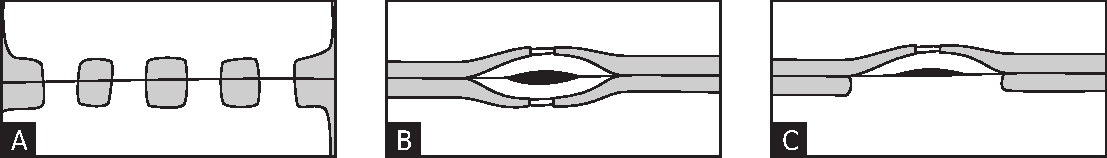
\includegraphics[scale=0.7]{img/ch3_ponctuations2}
\caption{Ponctuations (A) simples (B) aréolées; (C) semi-aréolées; Image préparée par Julie Ferland pour \cite{achim2010dendroecologie}}
\label{fig:ponctuations2}
\end{figure}


\begin{figure}[h]
	\centering
	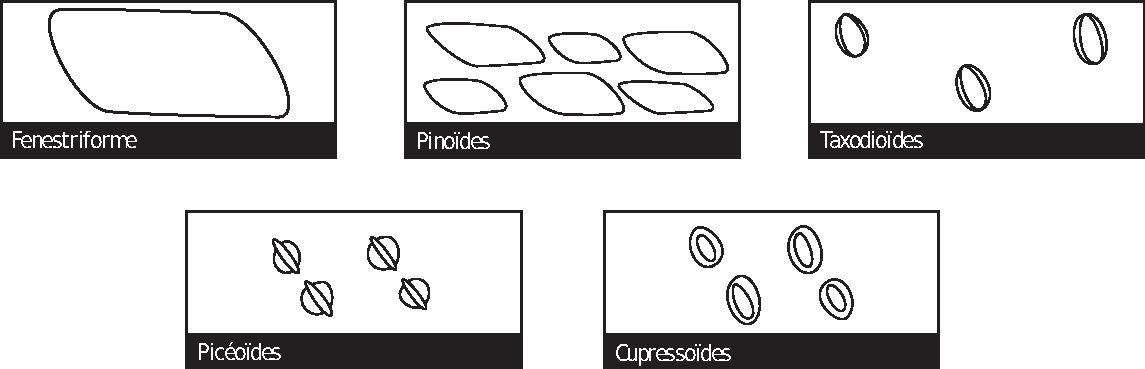
\includegraphics[scale=0.7]{img/ch3_ponctuations}
	\caption{Ponctuations des champs de croisement. Image préparée par Julie Ferland pour \cite{achim2010dendroecologie}}
	\label{fig:ponctuations}
\end{figure}
	
\subsubsection{Ponctuations fenestriformes}

Grandes ponctuations de forme quadrangulaire présentes chez certains pins (pin blanc et pin rouge par exemple).

\subsubsection{Ponctuations pinoïdes}

Ponctuations plus petites que les ponctuations fenestriformes et plus nombreuses par champs de croisement. L'aréole peut ne pas être visible dans le bois initial. Elles sont caractéristiques du groupe des pins durs.

\subsubsection{Ponctuations picéoïdes}

Petites ponctuations à ouverture étroite, linéaire et semblant déborder l'aréole. Elles sont caractéristiques des épinettes, des mélèzes, du sapin Douglas et des pruches.

\subsubsection{Ponctuations taxodioïdes}

Ponctuations à ouverture ovale à circulaire tangente en deux points au contour de l'aréole. L'aréole est étroite mais bien visible. Elles sont caractéristiques du séquoia, des sapins et des thuyas.

\subsubsection{Ponctuations cupressoïdes}

Ponctuations semblables aux picéoïdes mais l'ouverture est elliptique et entièrement incluse dans l'aréole. Elles sont caractéristiques du genévrier, des cyprès (\textit{Chamaecyparis spp.}) et présentes à l'occasion chez les épinettes et les pruches.

\begin{figure}[h]
	\centering
	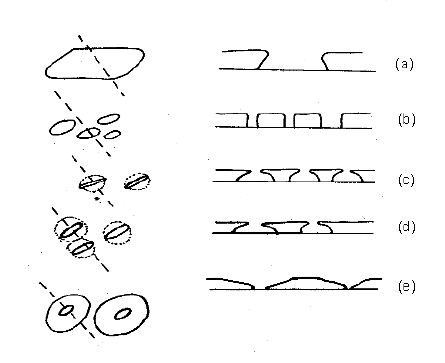
\includegraphics[scale=0.6]{img/ch3_pontuations_cote}
	\caption{Ponctuations des champs de croisement en plan tangentiel a) fenestriformes; b) pinoïdes; c) picéoïdes; d) cupressoïdes; e) taxodioïdes; (d’après \cite{butterfield2012three})}
	\label{fig:pontuations_cote}
\end{figure}

\section{L'anatomie du bois des résineux en un clin d'œil}

La figure~\ref{fig:Fahn} illustre l'organisation des différentes cellules du bois des résineux.

\begin{figure}[h]
\centering
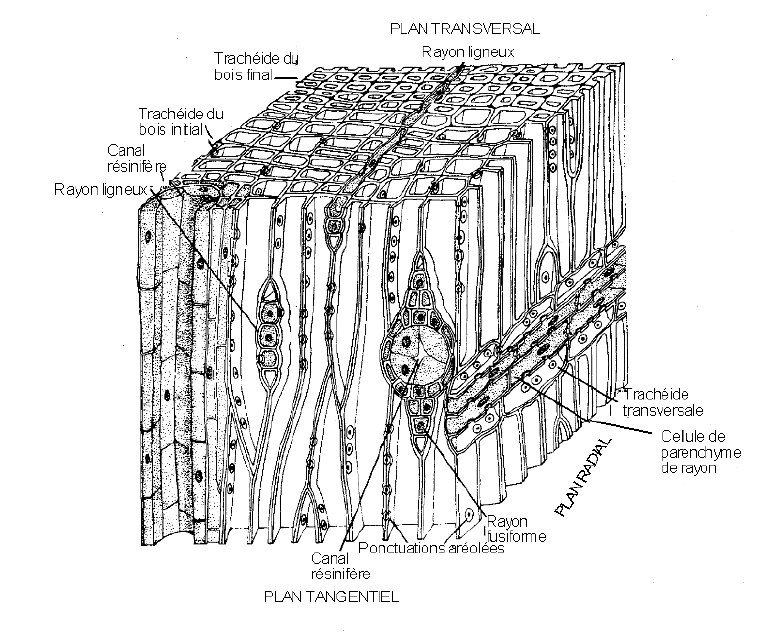
\includegraphics[scale=0.7]{img/ch3_Fahn}
\caption{Structure tridimensionnelle générale des résineux (adapté de \cite{fahn1990plant})}
\label{fig:Fahn}
\end{figure}




%Références
%
%Butterfield, B.G.; Meylan, B.A. 1980. Three-dimensional structure of wood. An ultrastructural approach. Second edition. Chapman and Hall, London, New York. 103 p.
%
%Fahn, A. 1990. Plant anatomy. Fourth edition. Pergamon Press, Oxford. 588 p.
%
%Hoadley, R.B. 1990. Identifying wood. Accurate results with simple tools. The Taunton Press Inc. Connecticut, USA. 223 p.
